\section{Event preselection}
\label{sec:vlq:presel}
Events satisfying the trigger selection described in section \ref{chp:sec:data} are further classified into the ``1-lepton'' or ``0-lepton'' channels depending on the multiplicity of the selected leptons. Events in the 1-lepton channel are required to have exactly one reconstructed electron or muon satisfying the quality and kinematic criteria discussed in sections \ref{chp:obj:sec:ele} and \ref{chp:obj:sec:muon}. The selected lepton is required to match the lepton reconstructed by the single-lepton trigger with $\Delta R<0.15$. 
The lepton is required to have $\pt>25$ $\gev$ in order to be in the region where the trigger is fully efficient. Events satisfying either the electron or muon selections are combined and treated coherently, regardless of the lepton flavour. Events in the 0-lepton channel are required to satisfy the \MET trigger and to have \MET >200 $\gev$ in order to be in the region where the trigger is fully efficient. Events are required to have $\ge$5 ($\ge$6) jets with $\pt$ > 25 $\gev$ and $|\eta|<2.5$ in the 1-lepton (0-lepton) channel. Given the high number of $b$-quarks in the final state for signal events, a requirement of at least two $b$-tagged jets ($77\%$ operating point) is included for both channels to remove backgrounds not including $b$-quark jets. Additional requirements are related to the quality of the event reconstruction or the detector status and are usually referred to as ``event cleaning'':

\bi
\ib Data quality:  the ``Good Runs List'' is the collection of lumiblocks\footnote{A luminosity block (lumiblock) is the smallest unit of time in the ATLAS data-taking defined as the minimal period where all the data-taking configurations are constant. In general the duration of a luminosity block is of the order of 1 minute.} with no subdetector problems; thus only events present in this list are retained.
\ib Corrupted data removal: detector problems happening for periods shorter than a lumiblock are rejected with event-level flags without losing the entire lumiblock. Events are removed if integrity problems or noise bursts are found in the calorimeters or if  they are affected by the recovery procedure for single-event upsets in the SCT.
\ib Bad jets removal: events are rejected if a ``bad jet'', as defined in section \ref{chp:obj:sec:jet:cleaning}, with $\pt > 20\,\gev$ and $|\eta|$ < 2.5 is found. This condition is particularly important to minimise the contribution from mismeasured jets to the \MET computation.
\ei

In the 1-lepton channel the presence of a leptonically-decaying $W$ boson in the final state can also be exploited to suppress background from multijet events, which are characterised by a fake lepton. The transverse mass of the leptonic $W$ boson, $m_{\rm T}^{W}$, can be reconstructed from the lepton and the \MET:

\be
m_{\rm T}^{W}= \sqrt{2p_{T}^{\ell} \MET (1-\cos\Delta \phi(\ell,\MET))},
\label{sec:vlq:eq:mtw}
\ee

\noindent where $\pt^{\ell}$ is the transverse momentum (energy) of the muon (electron) and $\Delta \phi$ is the azimuthal separation between the lepton and the direction of the missing transverse momentum. Thus, additional requirements are made on \MET and $m_{T}^{W}$: \MET>20 $\gev$ and \MET + $m_{T}^{W}$ > 60 \gev.\par Multijet events in the 0-lepton originate from mismeasured high-$\pt$ jets resulting in large \MET that tends to be aligned with the jet direction. A requirement of $\Delta \phi_{\rm min}^{4j}>0.4$ is made to suppress it (see figure \ref{sec:vlq:fig:dphi}), where $\Delta \phi_{\rm min}^{4j}$ is the minimum azimuthal separation between the \MET vector and the four highest-$\pt$ jets. This requirement  is very effective to suppress multijet events at negligible level. Figure \ref{sec:vlq:fig:dphimeff} show the $m_{\rm eff}$\footnote{Defined in section \ref{sec:vlq:discrvar}. } distribution before and after the $\Delta \phi_{\rm min}^{4j}$ cut, which suppresses the multijet background and improves data-to-MC agreement.


\begin{figure}[t!]
  \centering
  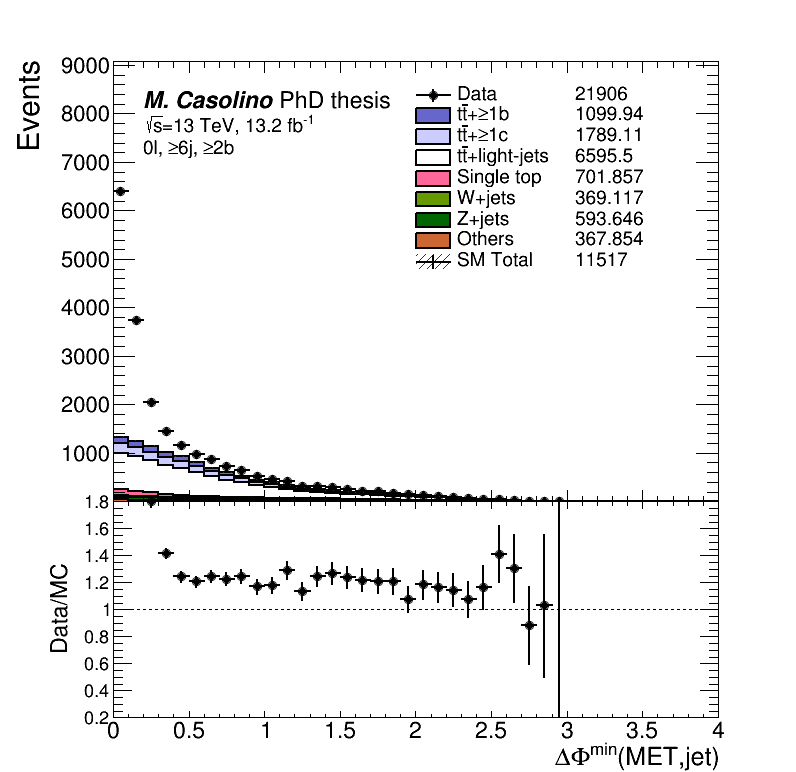
\includegraphics[width=0.5\textwidth]{figures/VLQ/canv_c0l2b_dPhi_jetmet.png}
 \captionsetup{width=0.85\textwidth} \caption{\small Distribution of $\Delta \phi_{min}^{4j}$ at preselection level prior to cutting on this variable.}
  \label{sec:vlq:fig:dphi}
\end{figure}


\begin{figure}[t!]
\begin{subfigure}{0.5\textwidth}
  \centering
  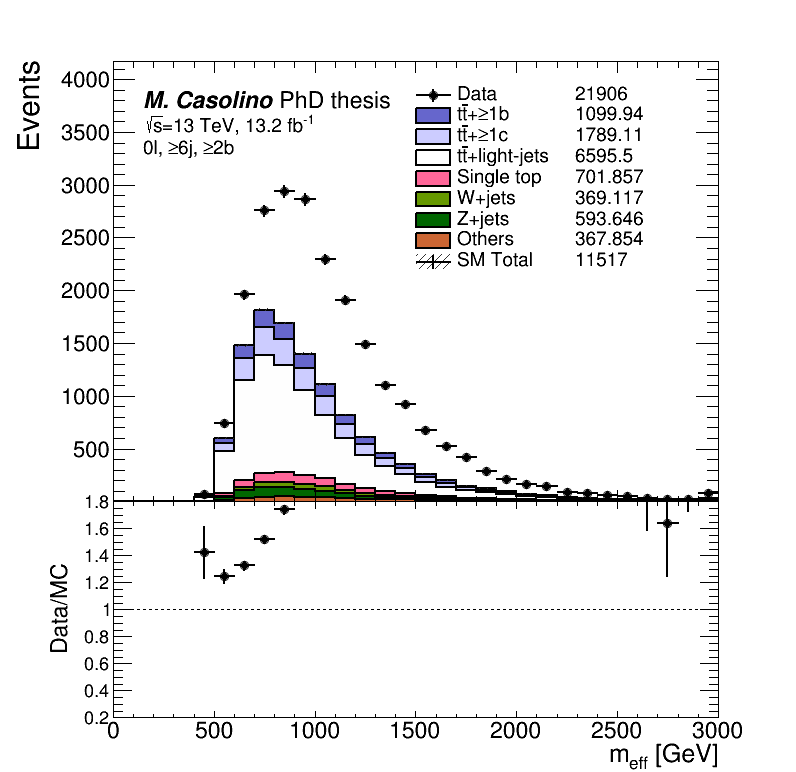
\includegraphics[width=0.9\textwidth]{figures/VLQ/canv_c0l2b_meff_nodPhi.png}
  \caption{}
  \label{}
\end{subfigure}
\begin{subfigure}{0.5\textwidth}
  \centering
  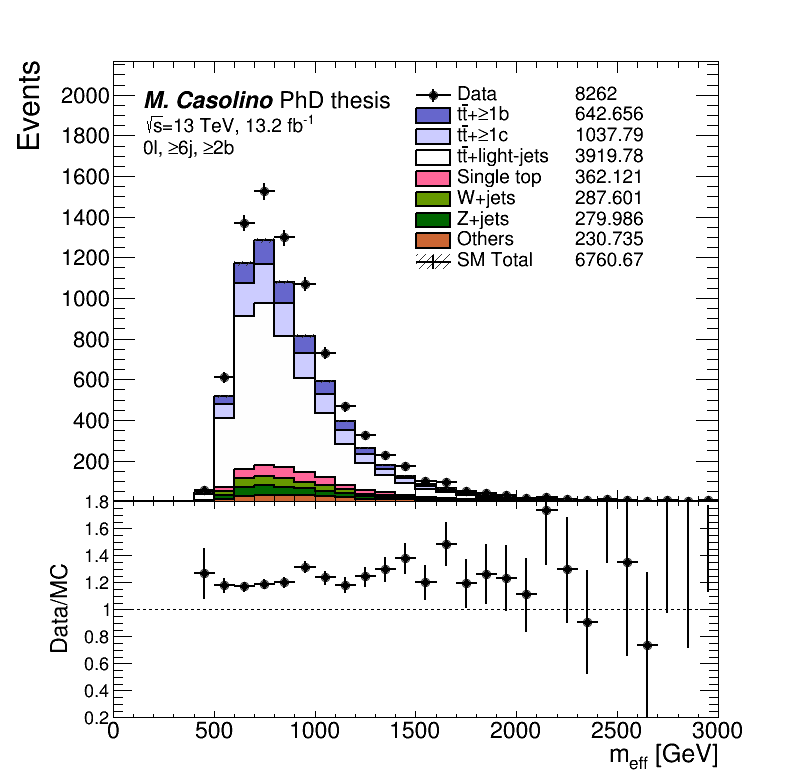
\includegraphics[width=0.9\textwidth]{figures/VLQ/canv_c0l2b_meff_afterdPhi.png}
  \caption{}
  \label{}
\end{subfigure}
\captionsetup{width=0.85\textwidth} \caption{\small $m_{\rm eff}$ distribution (a) before and (b) after the $\Delta \phi_{min}^{4j}>0.4$ cut.}
\label{sec:vlq:fig:dphimeff}
\end{figure}


 Table \ref{tab:vlq:presel} summarises the requirements described above and referred to as the ``preselection''.

\begin{table}[t!]\footnotesize
\begin{center}
\begin{tabular}{c|c|c}
  \hline \hline
  \multicolumn{3}{c}{Preselection requirements}\\
  \hline
   Requirement & 1-lepton channel & 0-lepton channel \\
  \hline
  Event cleaning & \checkmark & \checkmark\\
  Trigger & Single-lepton trigger & \MET trigger\\
  Leptons & =1 isolated e or $\mu$ & =0 isolated e or $\mu$ \\
  Jets & $\ge$5 jets & $\ge$6 jets\\
  $b$-tagging & $\ge$2 $b$-tagged jets &$\ge$2 $b$-tagged jets\\
  \MET & \MET > 20 \gev & \MET > 200 \gev \\
  Other \MET-related & \MET + $m_{\rm T}^{W}$ > 60 \gev& $\Delta \phi_{\rm min}^{4j}>0.4$\\  
 \hline \hline
\end{tabular}
\captionsetup{width=0.85\textwidth} \caption{\small Summary of preselection requirements for the 1-lepton and 0-lepton channels. Here $m_{\rm T}^{W}$ is the transverse mass of the lepton and the \MET vector, and  $\Delta \phi_{\rm min}^{4j}$ is the minimum azimuthal separation between the \MET vector and the four highest-$\pt$ jets. }
\label{tab:vlq:presel}
\end{center}
\end{table}

%\clearpage
 